%---------- Inleiding ---------------------------------------------------------

\section{Introductie}%
\label{sec:introductie}

Het implementeren van ETL's en ELT's spelen een kritieke rol in de development binnen Net IT. Doordat Net IT een Microsoft gebasseerd bedrijf is gaan we dus onderzoeken naar de mogelijkheden voor het implementeren van ETL's en ELT's binnen in Microsoft Azure. Momenteel gebruikt Net IT vooral Azure Data Factory en Azure Synapse Analytics. Hierbij wordt er gebruik gemaakt van de UI tools die Azure Data Factory aanbiedt. We gaan kijken of er andere mogelijkheden zijn om dit bijvoorbeeld via code te gaan doen (bijvoorbeeld in Azure Databricks). Deze gaan we dan gaan vergelijken in performantie, kostprijs (voor dezelfde performantie), complexiteit, moeilijkheidsgraad in opzet en configuratie van de resources (bicep templates), verschil in implementatietijd en mogelijkheden van de tool. De methode die gebruikt zal worden is een gemengde aanpak gebasseerd op literatuuronderzoek en het opstellen van proof-of-concepts. Dit zal resulteren in een rapport van aanbevelingen voor Net IT zodat men betere beslissingen kan maken bij het implementeren van ETL's en ELT's binnen in Microsoft Azure.

\section{State-of-the-art}%
\label{sec:state-of-the-art}

Als data data engineer krijgt men data in veel verschillende vormen. Het is dus noodzakelijk om deze data klaar te maken voor business analytics.~\autocite{Kromer2022} Hiervoor maakt men gebruik van ETL's en ELT's. Dit zijn processen die organisaties gebruiken voor het verzamelen en samenvoegen van data uit meerdere bronnen. Bij ETL's wordt de data getransformeerd voor het naar de doelopslagplaats geladen wordt, terwijl dit bij ELT's pas achteraf gebeurd. Daardoor staat ETL voor Extract, Transform and Load en ELT voor Extract, Load and Transform.~\autocite{Bartley2023} 

In Azure zijn er meerdere mogelijkheden voor het implementeren van ETL's en ELT's. Één van deze mogelijkheden is Azure Data Factory. Zoals te zien in de enquête van~\textcite{Sreemathy2021} is dit de meest populaire data integratie service die aangeboden wordt door de cloud providers. Binnen Azure Data Factory kan er gebruik gemaakt worden van Mapping Data Flows, dit is een codevrije manier waarmee ETL's opgebouwd kunnen worden. De logica achter de ETL kan hierna makkelijk getest worden op live data en samples.~\autocite{Kromer2022a} 

Daarnaast biedt Azure ook Azure Databricks aan. Het verschil hierbij is dat de ETL's worden geïmplementeerd via code terwijl dat bij Azure Data Factory via de UI tools kan gebeurt. Azure Databricks is gebasseerd op het Apache Spark open source project. Het grote voordeel is dat het platform het toelaat om makkelijker te kunnen samen werken. Daarnaast is Apache Spark niet enkel gelimiteerd tot het maken van ETL's maar kan het ook gebruikt worden voor Machine Learning etc.~\autocite{Etaati2019}

\section{Methodologie}%
\label{sec:methodologie}

\begin{center}
    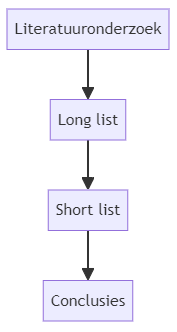
\includegraphics{graphics/methodologie.png}    
\end{center}


Onze eerste fase is het literatuuronderzoek. Hierbij gaan we gaan kijken welke mogelijkheden er zijn voor het implementeren van ETL's en ELT's binnen in Azure. Dit zullen we doen met behulp van academische onderzoekstools zoals bijvoorbeeld Google Scholar en andere relevante databanken en bronnen. Ook de documentatie van Azure, casestudies van bedrijven die gebruik maken van Azure en blogs van experts op dit vakgebied zullen hier zeker bij van te pas komen. Deze fase zal ook zeker in samenwerkingen met Net IT gebeuren zodat de huidige gebruikte technologieën voor het implementeren van ETL's en ELT's zeker niet uitgesloten worden. Dit onderdeel zal naar verwachting 4 weken in beslag nemen. 

In de tweede fase zullen we de resultaten van het literatuuronderzoek samenvatten in een long list. Op basis hiervan kunnen we dan verder gaan in ons onderzoek. Doordat dit een kleine fase is zal dit bij de tijd van de eerste fase horen.

In de derde fase zullen we op basis van de long list een proof-of-concept uitwerken voor elke mogelijkheid dat er binnen Azure is. We zullen een situatie opzetten met dummy data in een data lake. Het doel is dat er op basis van deze data export bestanden zullen gemaakt worden. We gaan kijken naar performantie, kostprijs, complexiteit, moeilijkheidsgraad in opzet en configuratie van de resources, verschil in implementatietijd en de mogelijkheden die de tool aanbied. We zullen de opties dan ook gaan vergelijken met elkaar. Belangrijk is dat de tests representatief zijn voor werkelijke implementaties binnen Net IT en dat deze ook zo nauwkeurig mogelijk gaan gebeuren. Dit zal resulteren in een short list van mogelijke opties die er zijn. Dit zal de langste fase zijn en zal dus 6 weken in beslag nemen.

De vierde en laatste fase, die naar verwachting twee weken zal duren, is de evaluatie van de opties die we hebben onderzocht. Het doel is om te tonen welke optie het beste is. Het kan zijn dat niet steeds één optie de beste is. Daardoor zal het resultaat van deze analyse een gedetailleerd vergelijkingsrapport zijn en aanbevelingen, per scenario, voor welke optie het beste zou kunnen zijn.


%---------- Verwachte resultaten ----------------------------------------------
\section{Verwacht resultaat, conclusie}%
\label{sec:verwachte_resultaten}

Het resultaat zal een gedetailleerd vergelijkingsrapport zijn met een overzicht van de meest veelbelovende implementatiemogelijkheden binnen Azure voor ETL's en ELT's. Het rapport zal niet alleen een overzicht bieden van de verschillende opties maar ook gedetailleerde richtlijnen per tool. Dit stelt Net IT in staat om niet alleen de beste optie te identificeren voor hun specifieke situatie maar ook om een dieper inzicht te krijgen in de operationele implicaties, kostenstructuur, etc. 

Het is belangrijk om op te merken dat de aanbevelingen flexibel zullen zijn en kunnen variëren naargelang wat voor ETL of ELT er zal geïmplementeerd moeten worden.


